%%%%%%%%%%%%%%%%%%%%%%%%%%%%%%%%%%%%%%%%%%%%%%%%%%%%%%%%%%%%%%%%%%%%
%% I, the copyright holder of this work, release this of into the
%% public domain. This applies worldwide. In some countries this may
%% not be legally possible; if so: I grant anyone the right to use
%% this work for any purpose, without any conditions, unless such
%% conditions are required by law.
%%%%%%%%%%%%%%%%%%%%%%%%%%%%%%%%%%%%%%%%%%%%%%%%%%%%%%%%%%%%%%%%%%%%

\documentclass[
    %twoside,   % Printed version
    %printed,   % Printed version
    digital,    % PC version
    oneside,    % PC version
    color,
    11pt,
    nocover,
    notable,
    nolof,
    nolot,
    final
  %% More options are listed in the user guide at
  %% <http://mirrors.ctan.org/macros/latex/contrib/fithesis/guide/mu/fi.pdf>.
]{fithesis3}
%% The following section sets up the locales used in the thesis.
\usepackage[resetfonts]{cmap} %% We need to load the a T2A font encoding
%\usepackage[utf8]{inputenc}
\usepackage[T1]{fontenc}  % T2a commented %% to use the Cyrillic fonts with Russian texts.
\usepackage[
  main=english, %% By using `czech` or `slovak` as the main locale
                %% instead of `english`, you can typeset the thesis
                %% in either Czech or Slovak, respectively.
  english, czech %german, russian, slovak %% The additional keys allow
]{babel}        %% foreign texts to be typeset as follows:
%%
%%   \begin{otherlanguage}{german}  ... \end{otherlanguage}
%%   \begin{otherlanguage}{russian} ... \end{otherlanguage}
%%   \begin{otherlanguage}{czech}   ... \end{otherlanguage}
%%   \begin{otherlanguage}{slovak}  ... \end{otherlanguage}
%%
%% For non-Latin scripts, it may be necessary to load additional
%% fonts:
%\usepackage{paratype}
%\def\textrussian#1{{\usefont{T2A}{PTSerif-TLF}{m}{rm}#1}}

%%
%% The following section sets up the metadata of the thesis.
\thesissetup{
    date          = \the\year/\the\month/\the\day,
    university    = mu,
    faculty       = fi,
    type          = mgr,
    author        = Michal Hajas,
    gender        = m,
    advisor       = {RNDr. Petr Švenda, Ph.D.},
    title         = {Analysis of pseudo-random number generators based on lightweight cryptographic primitives},
    TeXtitle      = {Analysis of pseudo-random number generators based on lightweight cryptographic primitives},
    keywords      = {randomness testing, cryptanalysis, block functions, lightweight cryptography, pseudo-radnom number generators},
    TeXkeywords   = {randomness testing, cryptanalysis, block functions, lightweight cryptography, pseudo-radnom number generators},
}


\thesislong{abstract}{%
Abstract to be done
}

\thesislong{thanks}{%
Thank all.


\vspace*{11cm}\noindent{}\hspace*{-0.1cm}
Computational resources were supplied by the Ministry of Education, Youth and Sports of the Czech Republic under the Projects CESNET (Project No. LM2015042) and CERIT-Scientific Cloud (Project No. LM2015085) provided within the program Projects of Large Research, Development and Innovations Infrastructures.\\\\%
%
We also acknowledge the support of Czech Science Foundation, the project GA16-08565S.
}

%% The following section sets up the bibliography.
\usepackage{csquotes}
\usepackage[              %% When typesetting the bibliography, the
  backend=biber,          %% `numeric` style will be used for the
  style=numeric,          %% entries and the `numeric-comp` style
  citestyle=numeric-comp, %% for the references to the entries. The
  sorting=none,           %% entries will be sorted in cite order.
  sortlocale=auto         %% For more unformation about the available
]{biblatex}               %% `style`s and `citestyles`, see:
%% <http://mirrors.ctan.org/macros/latex/contrib/biblatex/doc/biblatex.pdf>.
\addbibresource{thesis.bib} %% The bibliograpic database within
                          %% the file `example.bib` will be used.
\usepackage{makeidx}      %% The `makeidx` package contains
\makeindex                %% helper commands for index typesetting.



%% These additional packages are used within the document:
\usepackage{paralist}
\usepackage{amsmath}
\usepackage{amsthm}
\usepackage{amsfonts}
\usepackage{url}
\usepackage{menukeys}

\usepackage[]{algorithm2e}

% cref, has to be loaded after hyperref
\usepackage{hyperref}
\usepackage[noabbrev,capitalise]{cleveref}
% for long equation wrap
\usepackage{wrapfig}
% figure captions
\usepackage{caption}
% subcaption for 2 figures in one
\usepackage{subcaption}
% H figures
\usepackage{float}

% tables
\usepackage{tabularx}
% colored cells (cellcolor)
\usepackage{colortbl}

% my colours
\usepackage{xcolor}

\usepackage{listings}   % fancy code listings
\captionsetup[lstlisting]{singlelinecheck=false, margin=0pt, font={sf,sl,footnotesize}}

\usepackage{minted}

%% My own inputs:
% enabling new fonts support (nicer)
\usepackage{lmodern}
% better typeset of line ends and so (nicer)
\usepackage{microtype}

\thesisload{}

\usepackage{tikz}
\usetikzlibrary{shapes,arrows,positioning}
\usetikzlibrary{decorations.pathreplacing}


% package to make bullet list nicer
\usepackage{enumitem}
\setitemize{noitemsep,topsep=3pt,parsep=3pt,partopsep=3pt}

% intendation
\usepackage{parskip}

% table colours
\newcommand{\fd}{\cellcolor{red!25}}
\newcommand{\fn}{}

% make captions italic
\usepackage[format=plain,
            font=it]{caption}

% Lubo's hack for margins
	\newcommand{\lmar}{3cm} % PC
	\newcommand{\rmar}{3cm} % PC
	\newcommand{\tmp}{3cm}  % PC

	%\newcommand{\lmar}{3.5cm} % Printed
	%\newcommand{\rmar}{2.5cm} % Printed
	%\newcommand{\tmp}{2.5cm}  % Printed


\usepackage[top=3cm, bottom=3.5cm, left=\lmar, right=\rmar]{geometry}

% Eliminates margins
\def\nomar{\list{}{\rightmargin-\tmp \leftmargin-\tmp}\item[]}
\let\endnomar=\endlist

% rotate figures
\usepackage{rotating}

% Table rotations
\usepackage{booktabs} % http://ctan.org/pkg/booktabs
\usepackage{xparse}   % http://ctan.org/pkg/xparse
% Rotation: \rot[<angle>][<width>]{<stuff>}
\NewDocumentCommand{\rot}{O{45} O{1em} m}{\makebox[#2][l]{\rotatebox{#1}{#3}}}%

% Rotates table cell
\newcolumntype{R}[1]{>{\begin{turn}{90}\begin{minipage}{#1}}l%
<{\end{minipage}\end{turn}}%
}

\crefname{formula}{Formula}{Formulas}

\renewcommand\_{\textunderscore\allowbreak}

\usepackage{pifont}% http://ctan.org/pkg/pifont
\newcommand{\cmark}{\ding{51}}%
\newcommand{\xmark}{\ding{55}}%

\begin{document}

% English indentation, vertical, not horizontal
\setlength{\parskip}{5pt}
\setlength{\parindent}{0pt}

%% We will define several mathematical sectioning commands.
\newtheorem{theorem}{Theorem}[section] %% The numbering of theorems
                               %% will be reset after each section.
                               
\newtheorem{formula}[theorem]{Formula}     %% The numbering of lemmas
%\newtheorem{corr}[theorem]{Corrolary}  %% and corrolaries will
                                %% share the counter with theorems.
%\theoremstyle{definition}
%\newtheorem{definition}{Definition}
%\theoremstyle{remark}
%\newtheorem*{remark}{Remark}

\chapter{Introduction}
\label{chap:introduction}


\chapter{Pseudo-Random number generators}

Random number generator is everything which produces random outcome. In real world it might be a coin, dice, etc. In computer science we know two types of randomness generators: truly random number generators (TRNG) and pseudo-random number generators (PRNG). Computers itself are not capable of producing a truly random data. They need input from peripherals (human interaction, network interference, etc.) and hence production of a truly random data is expensive. For that reason, PRNGs were introduced. Those generators are based on algorithm which is inputted with small amount of data (seed) and produce seemingly random sequence. Notice that the sequence can be generated by anyone who knows the original algorithm and the seed. \cite{jakobsson2014theory}

\section{Properties of PRNGs}

Security of PRNG is based on seed; it should be kept secret and generated so that it is unpredictable and truly random.

The PRNG algorithm is based on deterministic function $f$. For obtaining $n$-th output from generator formula $X_n = f(X_{n - 1})$ is used, where $X_0$ denotes seed. Schema of generation is shown in \cref{fig:prng}. 

\begin{figure}[h]
	\centering
	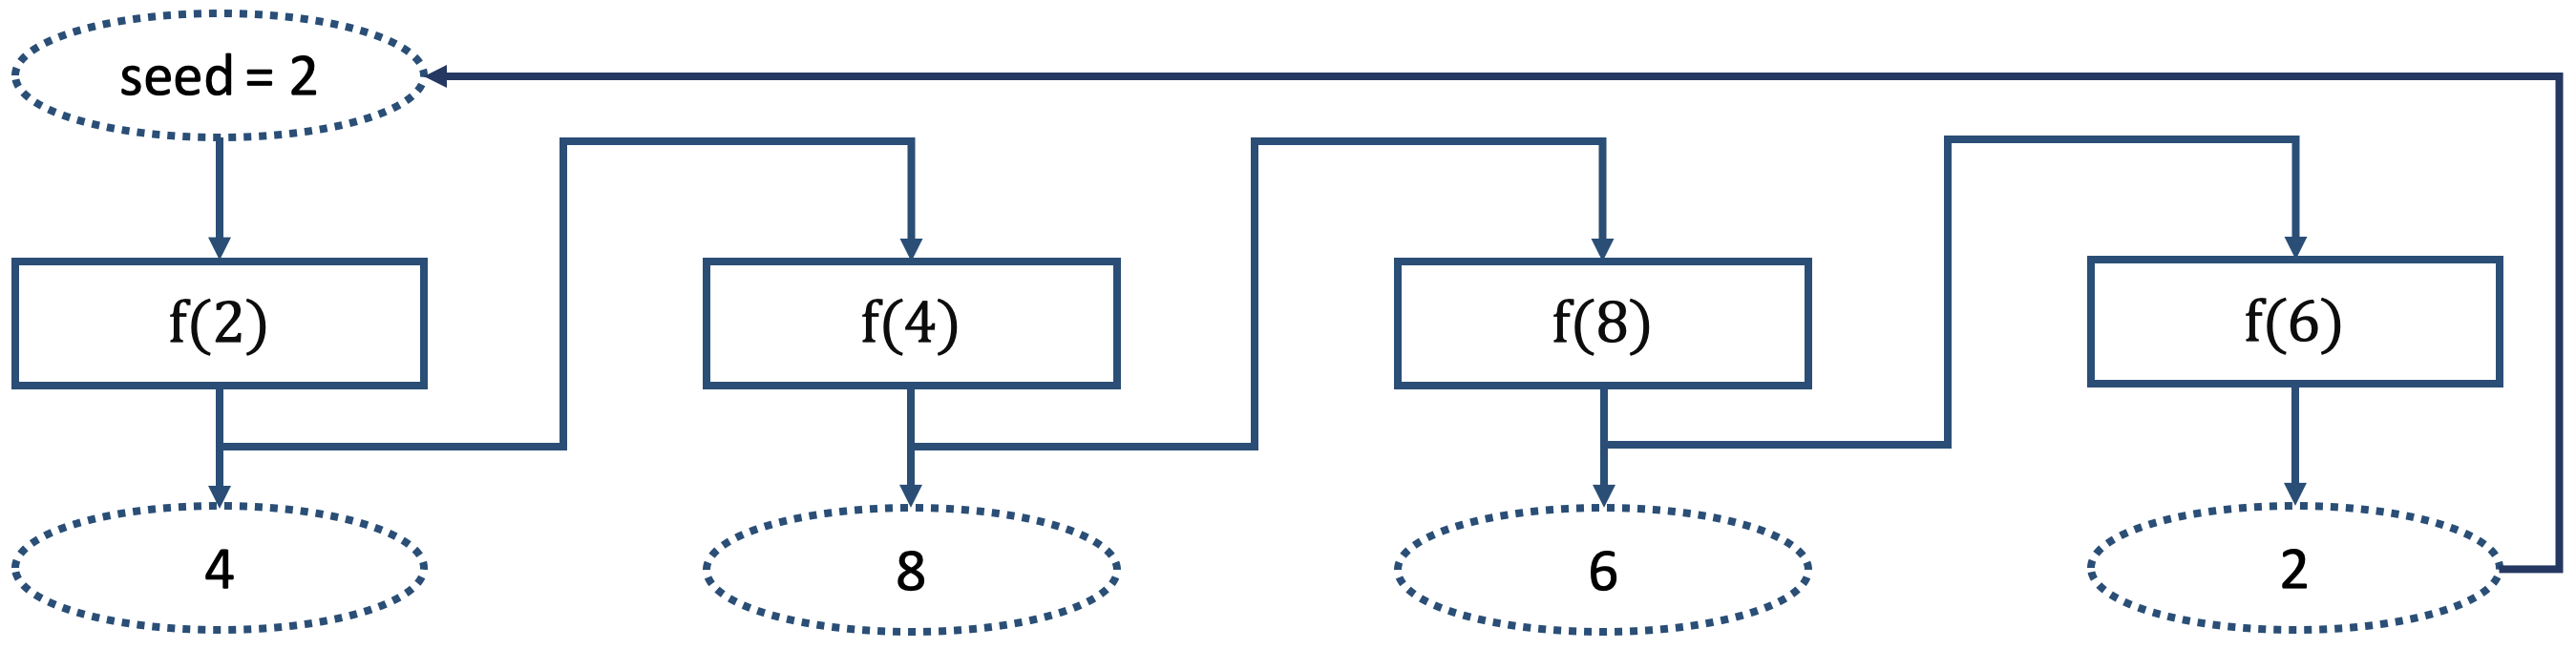
\includegraphics[width=0.8\textwidth]{./images/pictures/prng.png}
	\caption{Example of schema for linear congruential pseudo random number generator with function $f(X) \equiv \left(2 \times X~\bmod~10 \right)$. Period for this seed is four.}
	\label{fig:prng}
\end{figure}

The function $f$ is defined to take and produce sequences with fixed size (for example 4 bytes). This means there is finitely many options of inputs and corresponding outputs what eventually leads to repetitions. The number of iterations before first duplicity is called the \textit{period}. Generators are created so that the \textit{period} is maximized. When choosing PRNG for application the \textit{period} should be taken into account; it must be chosen so that the period is never reached. However, this can be achieved by regular reseeding with random data. A simple example of generator with period four is shown in \cref{fig:prng}.

Each sequence produced by PRNG must look random. This means it should pass all empirical tests of randomness (this is covered in \cref{sec:statistical-tests}). \cite{schneier1996applied}

For using PRNG within sensitive applications (such as cryptographic application) they need to fulfill one more requirement. It must be unfeasible to compute any information about following output given that the attacker knows all information about the previously generated sequence (including algorithm and hardware specification). Such generators are called cryptographically secure pseudo-random generators. \cite{schneier1996applied}

\section{Constructions techniques}

In this thesis we present following three categories of PRNGs.

\begin{description}
	\item[Simple (pure) generators.] The function $f$ is mostly some simple mathematical formula. Commonly known generator of this type is linear congruential generator (LCG). The formula is following. \cite{LEcuyer07testu01}
	
	\begin{equation}
	x_{n+1} = \left( a \times x_n + c \right)~~\bmod~~m
	\label{formula:lcg}
	\end{equation}	
	
	Where \textit{a, c, m} are fixed parameters for specific generator. Simple example of LCG is shown in \cref{fig:prng}. 

\end{description} 


SIMPLE (PURE), Stream ciphers, block/hash fncs

\section{Typical attacks}
Nextbit, prevbit, seed/state recovery

\section{Human cryptanalysis}

In this section, we present two cryptanalysis techniques. Both of them are very powerful; however, they are not fully automated. The cooperation with cryptanalyst is necessary. The first is Linear cryptanalysis which was introduced by Matsui \cite{matsui1993linear} in 1993 as a theoretical attack on Data Encryption Standard (DES). The other is differential cryptanalysis and was proposed by Biham and Shamir \cite{Biham1991} in 1991 with the same objective, to attack DES.


\subsection{Linear cryptanalysis}

It is one of the most famous known plaintext attacks against block ciphers; attacker knows some number of plaintext/ciphertext pairs, but he is not able to choose specific ones. 

The attack is based on building a linear approximation of part of a block cipher (non-linear), which consists of bits of plaintext, ciphertext, and key (round subkey). The general form of such approximation is following: 
\begin{equation}
\left( \bigoplus_{i \in \{1...b\}} P_{i} \right) \oplus \left( \bigoplus_{j \in \{1...b\}} C_{j} \right) = \left( \bigoplus_{k \in \{1...s\}} K_{k} \right)
\label{eq:general_approx}
\end{equation}
where $P_{i}$, $C_{j}$ and $K_{k}$ denote $i,j,k$-th bit of plaintext, ciphertext and key respectively. $\oplus$ stands for boolean \texttt{XOR} operator. Variables b and s are function specific and represent block size and key size. \cite{junod2000linear} 

Given such approximation and perfect cipher, the probability that this approximation holds should be $p = \frac{1}{2}$. Probability $p$ can be computed from the structure of investigated function. For purposes of the attack we need to find approximation which maximizes the bias $\epsilon = \lvert p - \frac{1}{2} \rvert$. 

The linear approximation can be used to perform two types of attacks:

\begin{description}
	\item[Obtaining one-bit information about the key.] Given the approximation in the form of \cref{eq:general_approx}, it is possible to obtain one-bit value of $X = \left( \bigoplus_{k \in \{1...s\}} K_{k} \right)$ following \cref{alg:one-bit}. \cite{junod2000linear}
	
	\begin{algorithm}[H]
		\KwData{$T$ denotes the number of results which equal to 0 when computing value of approximation for $N$ plaintext/ciphertext pairs.}

		\eIf{$T > \frac{N}{2}$}{

			$X = \begin{cases}
					0, & p > \frac{1}{2} \\
					1, & \text{otherwise}
				\end{cases}
			$
		}{
			$X = \begin{cases}
					1, & p > \frac{1}{2} \\
					0, & \text{otherwise}
				\end{cases}
			$
		}
		
		\caption{Obtaining one bit information about key using the linear approximation.} 
		\label{alg:one-bit}
	\end{algorithm}
	
	\item[Obtaining more bits of the key.] For demonstrating this type of attack, we will follow the tutorial from \cite{human-cryptanalysis} published by Howard M. Heys. He is attacking Substitution Permutation Network (SPN) defined within this paper. This function has four rounds; the size of subkey for each round and block is 16 bits. Each round consists of these operations: \texttt{mixing with subkey}, \texttt{substitution}, \texttt{permutation}. There are five subkeys because last round contains one more \texttt{mixing with subkey} at the end. Used notation is following.
	
	\begin{itemize}
		\item $K_{k,i}$ is an $i$-th bit of subkey for a $k$-th round. ($k \in \{1..5\}, i \in \{1..16\}$)
		\item $V_{j,i}$ is an $i$-th bit of output of a $j$-th round. ($j \in \{1..4\}, i \in \{1..16\}$)
		\item $U_{l,i}$ is an $i$-th bit of input to an $i$-th round. ($i \in \{1..4\}, i \in \{1..16\}$)
		
		$U_{i} = \begin{cases}
		P \bigoplus K_{1}, & i = 1 \\
		V_{i-1} \bigoplus K_{i}, & \text{otherwise}
		\end{cases}
		$
	\end{itemize}

	Heys is performing attack using 3-round approximation with probability either $p = \frac{15}{32}$ or $p = \frac{17}{32}$ based on specific subkeys. Key bits are omitted from the equation because the xor of all key bits results into fixed 0 or 1 bit which does not change resulting bias $\epsilon = \frac{1}{32}$. The approximation is following.   
	
	\begin{equation}
	U_{4,6} \oplus U_{4,8} \oplus U_{4,14} \oplus U_{4,16} \oplus P_{5} \oplus P_{7} \oplus P_{8} = 0
	\label{eq:linear-approximation-heys}
	\end{equation}
	
	Using this formula, it is possible to attack the last subkey $K_5$ by performing steps below.
	
	\begin{enumerate}
		\item Generate all possible options for subkey $K_{5}$ ($2^{16}$).
		\item For each of $N$ collected plaintext/ciphertext pair obtain bits of $U_{4}$ by reversing last round. 
		\item Apply the linear approximation (\cref{eq:linear-approximation-heys}) to captured bits and plaintext.
		\item For each subkey remember the number of pairs the approximation resulted with 0.  
		\item A subkey which ended up with a number which is most significantly different from $\frac{N}{2}$ is considered correct guess.
	\end{enumerate}
\end{description}

Using the linear cryptanalysis Matsui \cite{matsuiAttack} was able to break DES in the full number of rounds using $2^{43}$ random plaintext/ciphertext pairs.

\subsection{Differential cryptanalysis}

It is chosen plaintext attack; an attacker owns some number of plaintext/ciphertext pairs, and he can choose specific plaintexts. 

The attack is based on dependence between differences of two plaintexts and corresponding outputs. Differences are computed using exclusive xor operation of whole block, for example difference between two plaintexts $X_{1}$ and $X_{2}$ is denoted by $\Delta X = X_{1} \bigoplus X_{2}$. The difference between outputs $Y_{1}$ and $Y_{2}$ is expressed by $\Delta Y = Y_{1} \bigoplus Y_{2}$. In ideal case the probability $p$, of getting difference $\Delta Y$ for some  $\Delta X$, should be $\frac{1}{2^{n}}$ (differences should be equally distributed). 

The idea behind the attack is looking for the pair ($\Delta X$, $\Delta Y$) which maximizes the probability $p$ of obtaining difference $\Delta Y$ for plaintext $\Delta X$. The pair ($\Delta X$, $\Delta Y$) is called \textit{differential}.

Heys in his tutorial \cite{human-cryptanalysis} was simulating an attack using differential analysis with three round \textit{differential} ($\Delta U_{4}$ stands for a difference between inputs to fourth round). He found out that SPN for the plaintext difference $\Delta P = [0000$ $1011$ $0000$ $0000]$ results with $\Delta U_{4} = [0000$ $0110$ $0000$ $0110]$ with probability $\frac{27}{1024}$. Given this approximation it is possible to obtain bits of $K_{5}$ following steps below.

\begin{enumerate}
	\item Collect N plaintext pairs which satisfy chosen difference $\Delta P$.
	\item Generate all possible options for $K_{5}$ ($2^{16}$).
	\item For each plaintext pair and each option of key do following steps.
	\begin{enumerate}
		\item Reversely compute bits of $U_{4}$ for both corresponding ciphertexts using guessed key.
		\item For each key remember the number of times computed values give expected difference $\Delta U_{4}$.
	\end{enumerate}
	\item A key with the largest computed number is considered correct guess.
\end{enumerate}

DES in full round has been broken with complexity less than $2^{55}$. \cite{Biham1991}

\section{Distinguishers from truly random streams}
\label{sec:statistical-tests}

One of the most critical properties of output from cryptographic primitive is its indistinguishability from truly random data. Automatic tools for analyzing cryptographic primitives are based on this fact. Those tools rely on so-called empirical tests of randomness. Each tool contains several tests, where each of them has a different approach to testing. Mostly they are based on some property where there is a high probability that a truly random generator will satisfy this property. By comparing the expected and actual form of data, we can find out \textit{bias}. Higher the bias is, there is less probability that truly random generator outputted tested sequence.

Tests are based on testing a \textit{null hypothesis}, which is mostly formulated as data being tested are random. Those tests are based on probability; this means that even truly random data may end up with bad results from those tools. The output of each test is called \textit{p-value} which can be described as a probability that a truly random generator produces data which are less random than the data which were tested. We interpret the tests with respect to a significance level which is commonly known as $\alpha$. If the resulting \textit{p-value} is less than the significance level we say we rejected the hypothesis on significance level $\alpha$ (data are probably not coming from a truly random generator). The common value of $\alpha$ is 0.01. \cite{nist-explanation}

There are two types of errors which may occur during interpretation, Type I and Type II. Type I means that truly random data were rejected. The probability of Type I error is equal to significance level $\alpha$. When a tool does not reject data from a faulty generator, Type II error occurred. The probability of this error is denoted by $\beta$. However it is hard to compute the value of $\beta$ because there are many possible types of non-randomness which might occur. \cite{nist-explanation}

The example of the primary test often included in statistical test suites is a Monobit test, which is examining the uniformity of distribution of binary zeroes and ones bits within tested data. It is based on the fact, that there is a high probability that the amount of binary ones and zeroes is approximately the same assuming that each sequence occurs with same probability. A high-level view of this test is shown in \cref{fig:monobit}. 

\begin{figure}[h]
	\centering
	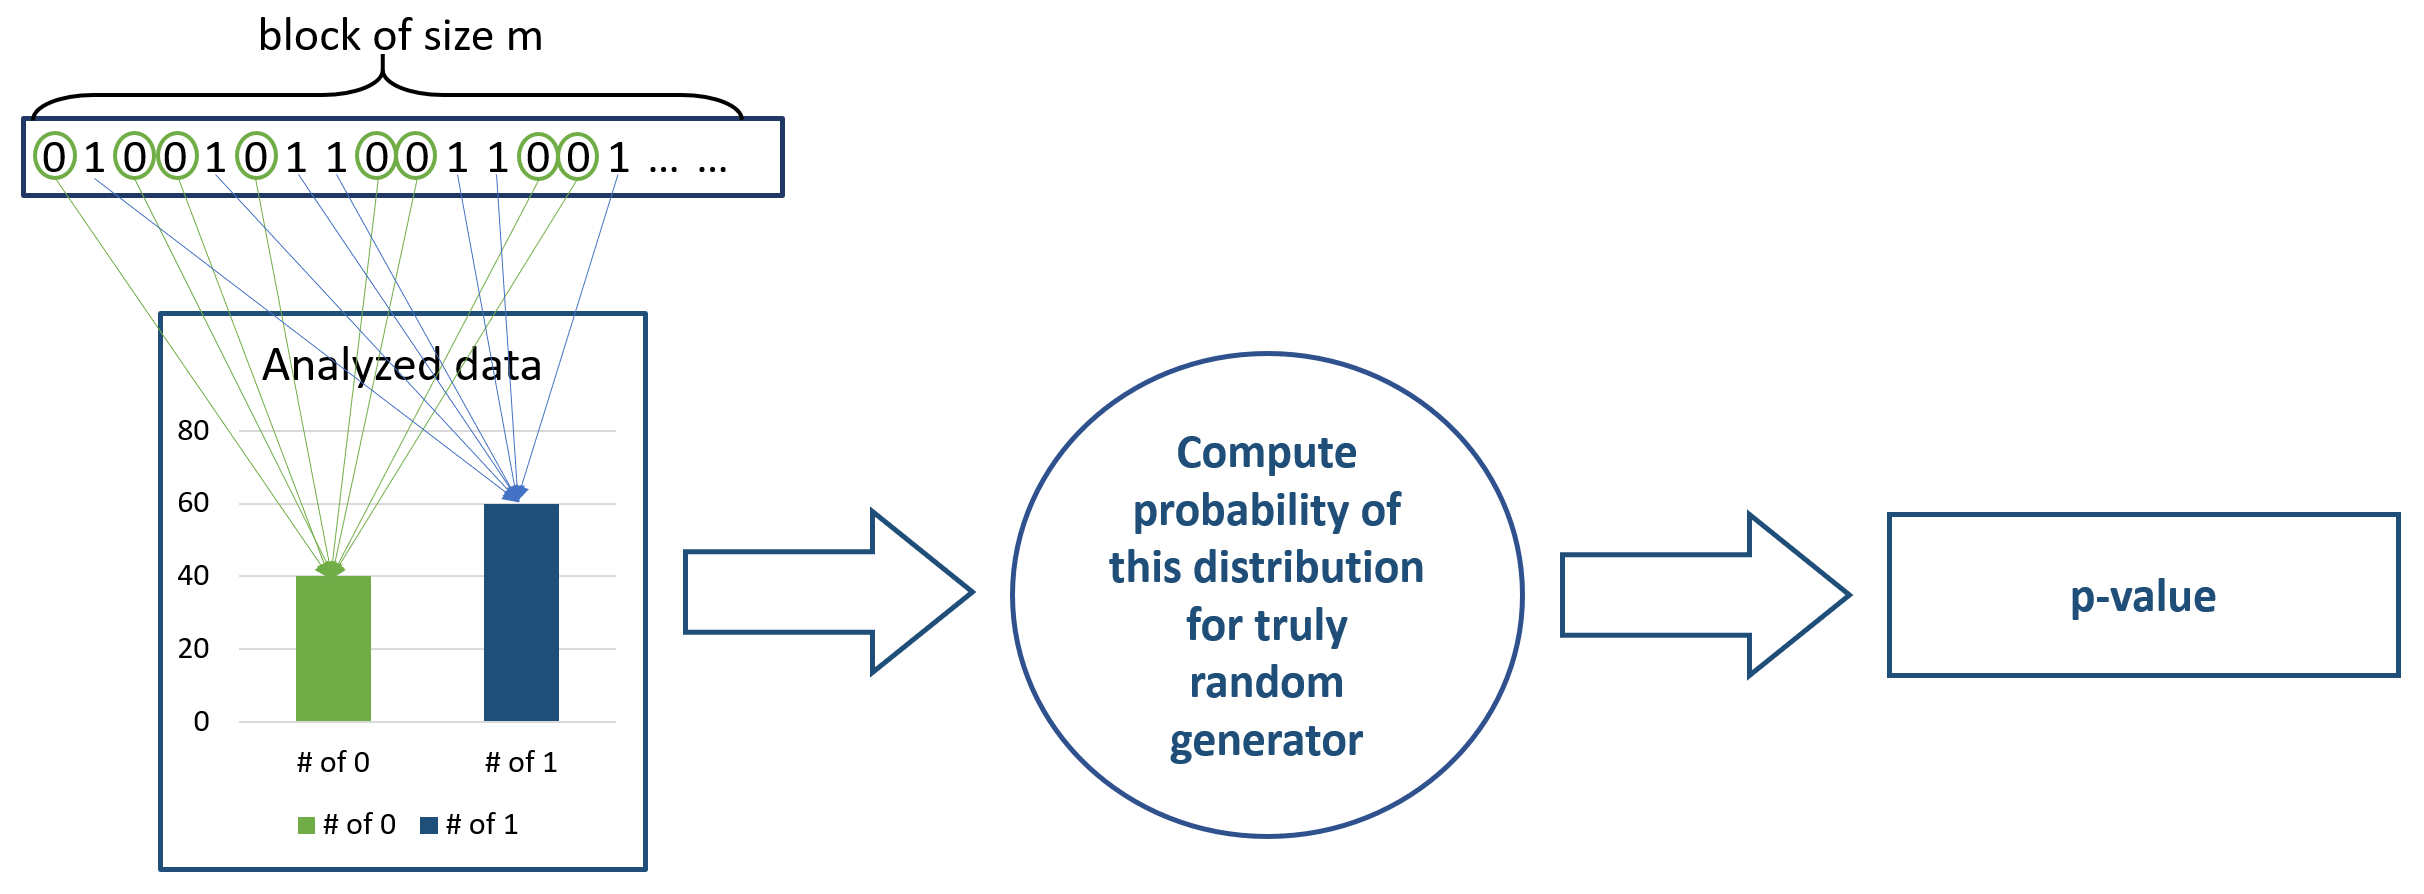
\includegraphics[width=0.9\textwidth]{./images/pictures/monobit-high-level.png}
	\caption{Monobit test from high level point of view.}
	\label{fig:monobit}
\end{figure}

\cref{fig:whole-suite} shows a high-level view of the whole test suite, where all tests are triggered. After evaluation of all tests, it is necessary to interpret the entire run of the battery of tests and make a final decision, whether investigated data are considered genuinely random or not. It is likely that even data with perfect properties will fail some of the tests. Our interpretation was not based only on the number of failed tests, but also on extremeness of test failures. For example, if there was one failed test within the whole test suite with an extreme p-value (less than $10^{-7}$), it is considered failure. However, if there were three failed tests with p-values close to $\alpha$ (not so extreme), it is still viewed as non-failure.

\begin{figure}[h]
	\centering
	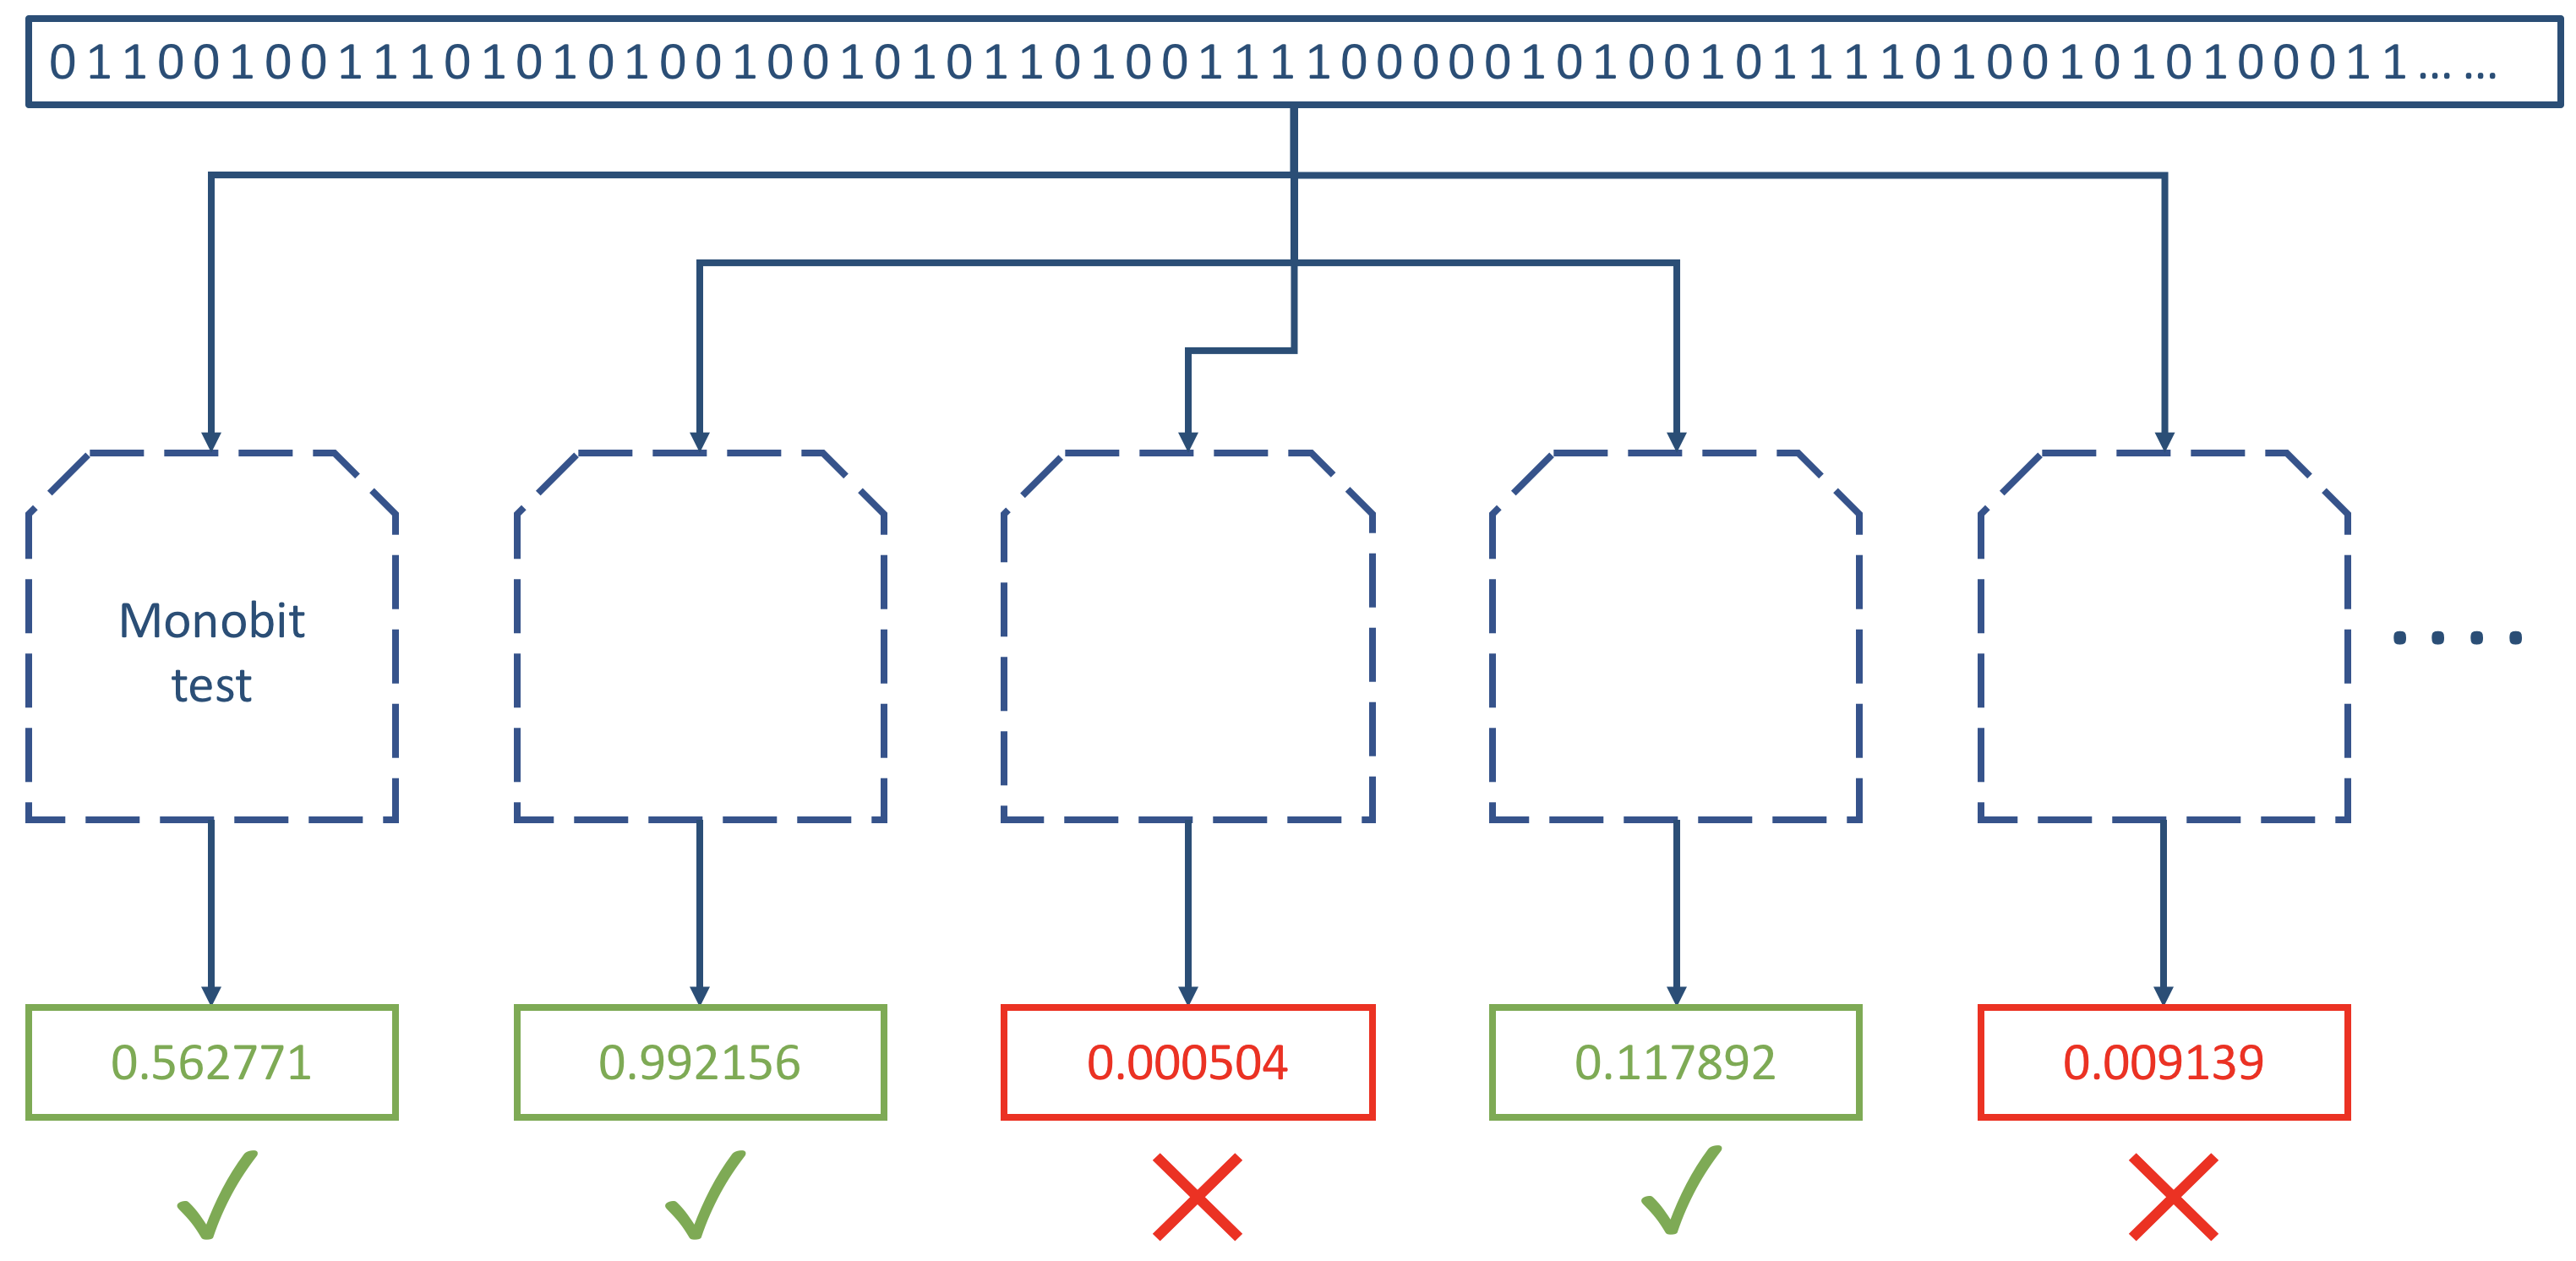
\includegraphics[width=0.9\textwidth]{./images/pictures/software-tool.png}
	\caption{High level view of software tool run.}
	\label{fig:whole-suite}
\end{figure}

\subsection{NIST STS}
{NIST STS}~\cite{nist-sts} is the most commonly used software tool for statistical analysis. It was developed by National Institute Of Standards and Technology (NIST) and is also part of FIPS 140-2~\cite{nist-fips-140-2} certification process. Even though the STS test suite is most commonly used, some of the other test suites generally have better results.

In this thesis we will not use original NIST implementation, instead of that we are using optimized version developed Marek Sýs and Zdeněk Říha which is approximately 50 times faster than reference implementation \cite{Sys:2016:A9O:2988516.2988228}. 

The tool contains 15 tests. However few of them have more variants. Therefore altogether 188 tests are executed within one run.

Dieharder~\cite{dieharder} is an extension of Diehard test suite \cite{diehard} developed by Robert G. Brown at Duke University. In the newest version, It contains together 31 tests. All tests from Diehard, three originates from NIST STS and the others are implemented by the author or come from different sources. However, not all tests will be used within this thesis. For choosing what tests to run we rely on project Randomness testing toolkit~\cite{Obratil2017thesis}.

\subsection{TestU01}

Pierre L'Ecuyer and Richard Simard introduced TestU01 software tool. The aim of this tool is the provision of the general and extensive set of software tools for statistical testing of random number generators. It contains a significant amount of tests, more than any other software tool we mentioned. Tests are organized into six batteries of tests. The battery of tests is a subset of tests, where each battery has a different purpose or time consumption. Batteries within TestU01 are divided into two categories, three of them designed for sequences of real numbers and the other for bit sequences.

For the first category there are batteries named \textit{SmallCrush}, \textit{Crush} and \textit{BigCrush}. \textit{SmallCrush} is fastest battery, hence it is recommended to start testing with this one and continue to \textit{Crush} only if sequence pass all tests. \textit{BigCrush} is longest one, it consumes 1414 times more time than \textit{SmallCrush} and 5 times more time than \textit{Crush} to test \textit{Mersenne Twister}~\cite{Matsumoto:1998:MTE:272991.272995} PRNG on a computer with AMD Athlon running at 2.4GHz. For binary sequences there are batteries \textit{Rabbit}, \textit{Alphabit} and \textit{BlockAlphabit}. \cite{l2007testu01}

Besides the batteries this software tool contains also some predefined pseudo-random number generators. Paper~\cite{l2007testu01} contains also results of those generators with batteries \textit{SmallCrush}, \textit{Crush} and \textit{BigCrush}.

\subsection{BoolTest}

BoolTest is simple but a strong testing tool developed by Marek Sýs et al. at the Centre for Research on Cryptography and Security, Masaryk University in Brno. It has a slightly different approach to randomness testing. The tool is based on a generalization of Monobit test. The main idea is looking for distinguisher between truly random and tested data in the form of boolean function. If a distinguisher is found the data are considered non-random otherwise random. The process starts with a division of sequence into blocks with size \textit{m}. The boolean function is in the form $f(x_{1}, x_{2}, \cdot \cdot \cdot, x_{m})$. Notice that Monobit test is specific case of this generalization with $m = 1$ and boolean function $f(x_{1}) = x_{1}$. 

Computation of success of distinguisher requires calculation of the value of the boolean function for each block so that $x_{k}$ is $k$-th bit of the block.
Expected number of computations which results with binary one is statistically computed and compared with actual results using Z-score statistic \cite{sheskin2003handbook}. This produces p-value. The more actual number of results which equals to one distinguish from the expected number, the better distinguisher we have.

Construction of distinguisher is based on the assumption that a combination of weaker and simpler boolean functions may lead to stronger distinguisher. The process starts with brute-force evaluation of all possible boolean functions of type  $f(x_{1}, x_{2}, \cdot \cdot \cdot, x_{m}) = x_{i}$ for $\forall i \in \{1, 2, \cdot \cdot \cdot, m\}$ with possibility to choose more complex functions in this phase. However, it cannot be too complicated as it is necessary to brute-force all possible functions. The second phase captures some number of best distinguishers which are then combined with XOR operation. This approach has two main advantages: it is possible to use precomputed values from the first phase, and it is possible to stop evaluation at any time when reasonably strong distinguisher is found. If no strong distinguisher is found tested data are considered random. \cite{booltest-secrypt2017}

\begin{figure}[h]
	\centering
	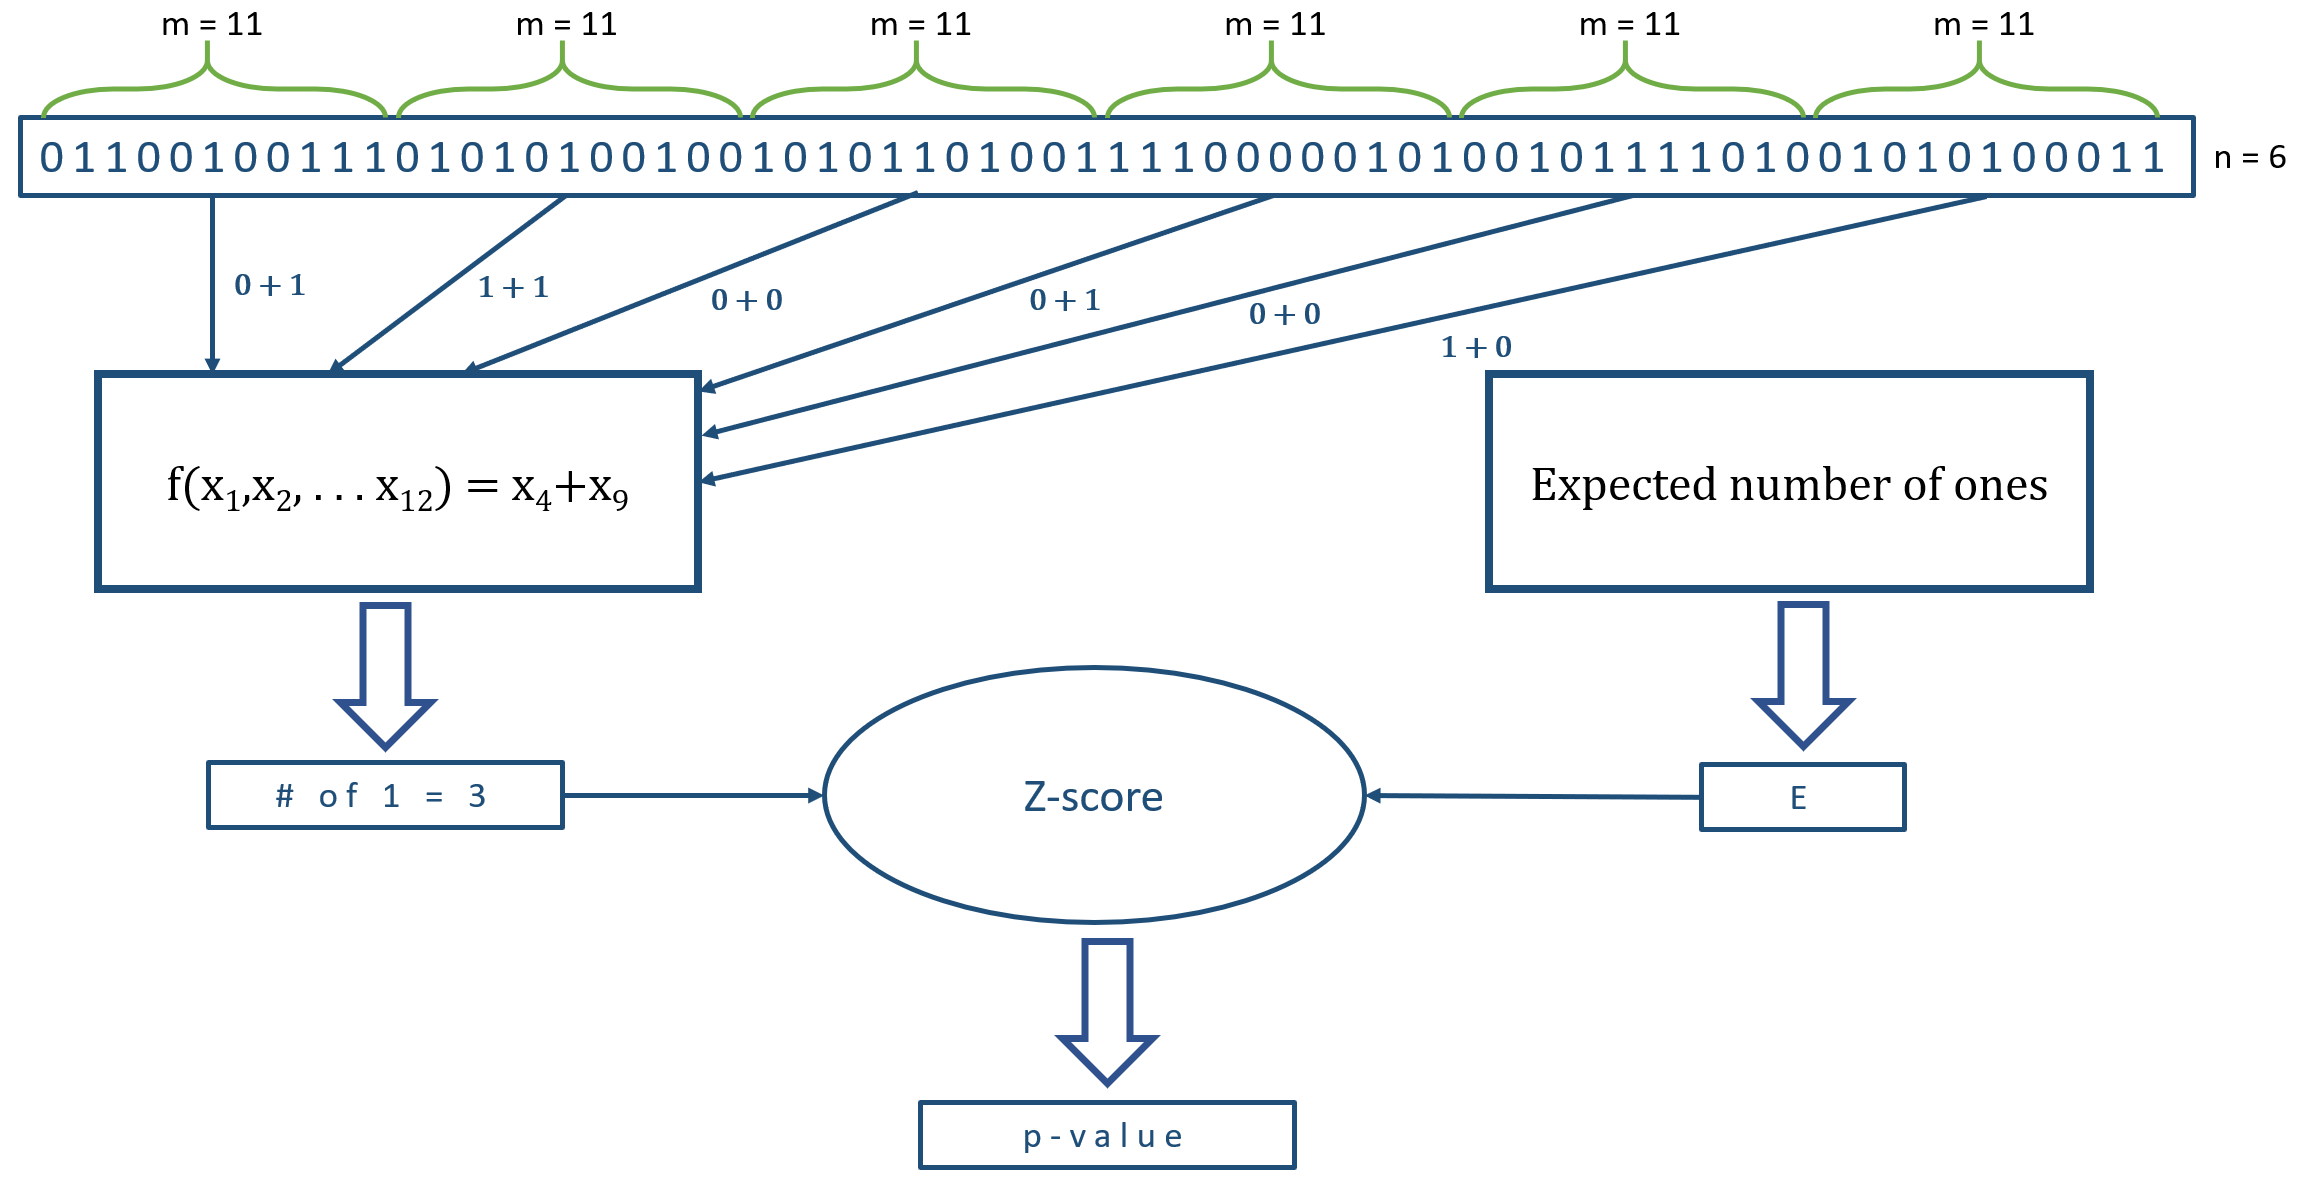
\includegraphics[width=0.8\textwidth]{./images/pictures/bool-test.png}
	\caption{Example of evaluation with BoolTest for sequence of size 72 bits with block size 12 and number of blocks 6. Evaluated boolean function (distinguisher) is $f(x_1,x_2, . . . x_{12}) = x_4+x_9$.}
	\label{fig:bool-test}
\end{figure}


\chapter{Introduction of CryptoStreams tool}
\label{chap:cryptostreams}

CryptoStreams tool is written in C++ language and is developed and maintained by team\footnote{The team of randomness testing involves following people: Radka Cieslarová, Michal Hajas, Dušan Klinec, Matúš Nemec, Jiří Novotný, Ľubomír Obrátil, Marek Sýs, Petr Švenda, Martin Ukrop and others.} at the Centre for Research on Cryptography and Security, Masaryk University~\cite{CryptoStreams}. The tool is used to generate a large amount of output data streams from parametrized cryptographic functions. Each stream is configurable with multiple options including output length, a structure of input plaintext, key, etc. 

\section{History}

An initial implementation of CryptoStreams project was part of tool EACirc~\cite{EACirc} which itself was a tool for automatic randomness testing based on genetic programming. At that moment it served only as a provider of testing data internally provided to its testing functionality and was not possible to use it separately outside of this project. We decided to split those two tools to provide flexible utilization with a broader range of tools in addition to EACirc. EACirc-streams project was introduced in 2017 and then in 2018 it was renamed to nowadays name, CryptoStreams.

\section{Idea}

The main idea behind CryptoStreams is an easy production of data from cryptographic primitives which are reduced in complexity, either by limiting the number of rounds or by providing them input with specific randomness properties, such as low Hamming weight, etc. The most significant advantage is that the tool contains a large number of cryptographic primitives such as block ciphers, hash functions, etc. All of them are integrated within a unified interface. CryptoStreams is also useful as an entry point for investigation of newly created cryptographic primitives, as it is built so that the addition of new primitives was as easy as possible. After obtaining data, it is possible to do any investigation over those data. For example, in this thesis, we conduct statistical analysis with seven statistical batteries of tests and also with a tool called BoolTest~\cite{booltest-secrypt2017}. Notice, that addition of new analysis tool requires no additional implementation on the side of CryptoStreams.

\section{Content of CryptoStreams}

In this section, we would like to present deeper details about what this tool provides. The tool currently contains four types of cryptographic primitives: block ciphers, hash functions, stream ciphers, and pseudo-random number generators. \cref{table:all-cryptoprimitives} shows counts of functions of corresponding types. First cryptographic primitives which were added to CryptoStreams were candidates from SHA-3 and eStream competitions. Those additions were done by Ondrej Dubovec~\cite{Dubovec2012thesis} and Matej Prišťák~\cite{Pristak2012thesis} in 2012. Within those theses were added 34 hash functions and 27 stream ciphers. Another addition was done by Martin Ukrop in his master thesis~\cite{Ukrop2016thesis} regarding authenticated encryption systems from CAESAR competition~\cite{caesar-competition}. Well known block ciphers like AES, DES, etc. were added by Karel Kubíček~\cite{Kubicek2017thesis} and Tamás Rózsa~\cite{Rozsa2018thesis} in their theses. The tool also contains a lot of other cryptographic primitives added outside of theses or papers.

% TODO: find citations for SHA-3 and eStream competition
\begin{table}[t]
	\centering	
	\begin{tabular}{|c|c|}
		\hline
		\textbf{\large Cryptographic primitive type} &  \textbf{\large Number of functions} \\ \hline
		Block ciphers  & 42 \\ \hline
		Hash functions & 51 \\ \hline  
		Stream ciphers & 27 \\ \hline
		PRNGS 		   & 6  \\ \hline		
	\end{tabular}
	\caption{List of all types of cryptographic primitives contained within CryptoStreams with the corresponding number of functions.}
	\label{table:all-cryptoprimitives}
\end{table}

Each output is generated by so-called \textit{streams} which are producers of data. Each call produces a chunk of data with configured size. Retrieving data from \textit{stream} in a loop and storing them, results in a data file with desired binary data. By configuring the size of chunk and number of chunks to save it is possible to set the size of resulting file. CryptoStreams contains the following types of streams.

\begin{description}
	\item[\textit{Streams} outputting data with static structure] which are mostly used as an input \textit{streams} such as plaintext or key. Those might be for example binary zero, binary one \textit{stream} or low Hamming weight stream (small amount of ones), etc. Pseudo-random streams also belong to this category. \cref{fig:static-stream} shows example of schema of such \textit{stream}.
	
	The list of static streams is following:  \texttt{dummy\_stream, true\_stream, false\_stream, mt19937\_stream, pcg32\_stream, counter, random\_start\_counter, sac, sac\_fixed\_position, sac\_2d\_all\_position} and \texttt{hw\_counter}. 

	
	\begin{figure}[h]
		\centering
		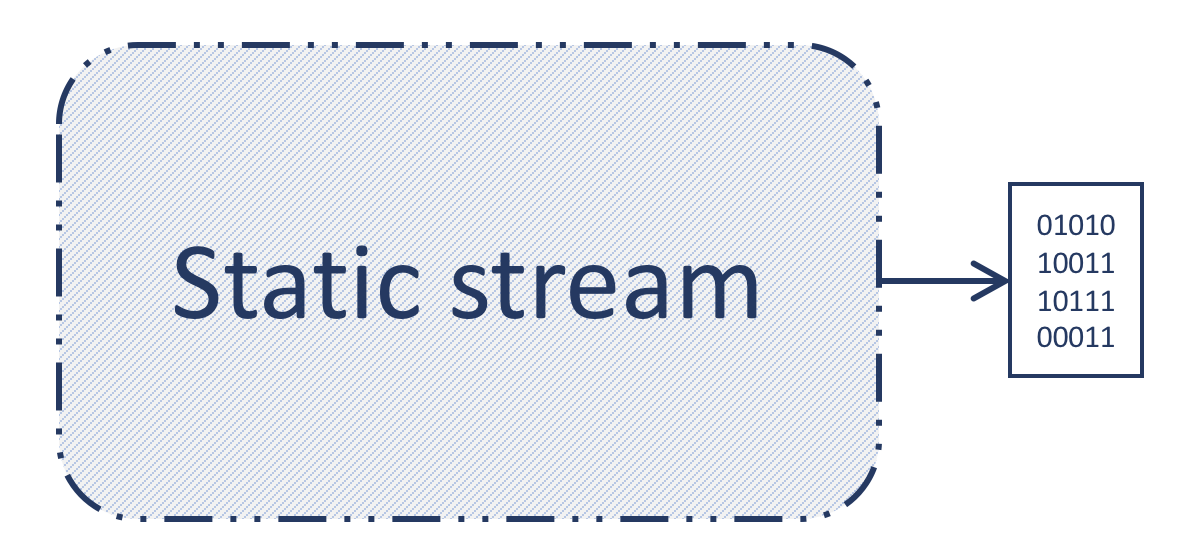
\includegraphics[width=0.5\textwidth]{./images/pictures/static-stream.png}
		\caption{Example of one call of static \textit{stream}.}
		\label{fig:static-stream}
	\end{figure}

	\item[Manipulating \textit{streams}] are configured with one or more inputs and manipulate them in a stream-specific way. For example, \textit{repeating stream} is repeating one output specified number of times before generating a new chunk of data from input \textit{stream}. Another example is \textit{tuple stream} that is getting more \textit{streams} as an input and for each call it returns chunk which contains data from each \textit{stream} concatenated together. Schema of this \textit{stream} is shown in \cref{fig:manipulating-stream}. Using tuple stream, it is possible to receive data which consists of plaintexts followed by corresponding ciphertexts.
	
	Currently implemented streams within this category are: \texttt{ single\_value\_stream, repeating\_stream} and \texttt{tuple\_stream}.
	
	\begin{figure}[h]
		\centering
		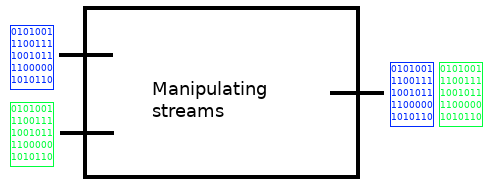
\includegraphics[width=0.7\textwidth]{./images/pictures/manipulating-stream.png}
		\caption{Example of one call from manipulating \textit{stream}, specifically \textit{tuple stream}. }
		\label{fig:manipulating-stream}
	\end{figure}
	
	\item[\textit{Streams} based on round-reduced cryptographic primitives.] Besides the round limitation it is also possible to configure them with various types of plaintext, key and initialization vectors inputs. \cref{fig:crypto-stream} shows a scheme of such stream which uses block cipher. The scheme may be different for other cryptographic primitives, for example, hash functions do not need key or iv as an input.
	
	Project contains 3 types of cryptoprimitves: \texttt{block\_ciphers, stream\_ciphers} and \texttt{hash\_functions}. Number of functions wihitn corresponding category is shown in \cref{table:all-cryptoprimitives}.
	
	\begin{figure}[h]
		\centering
		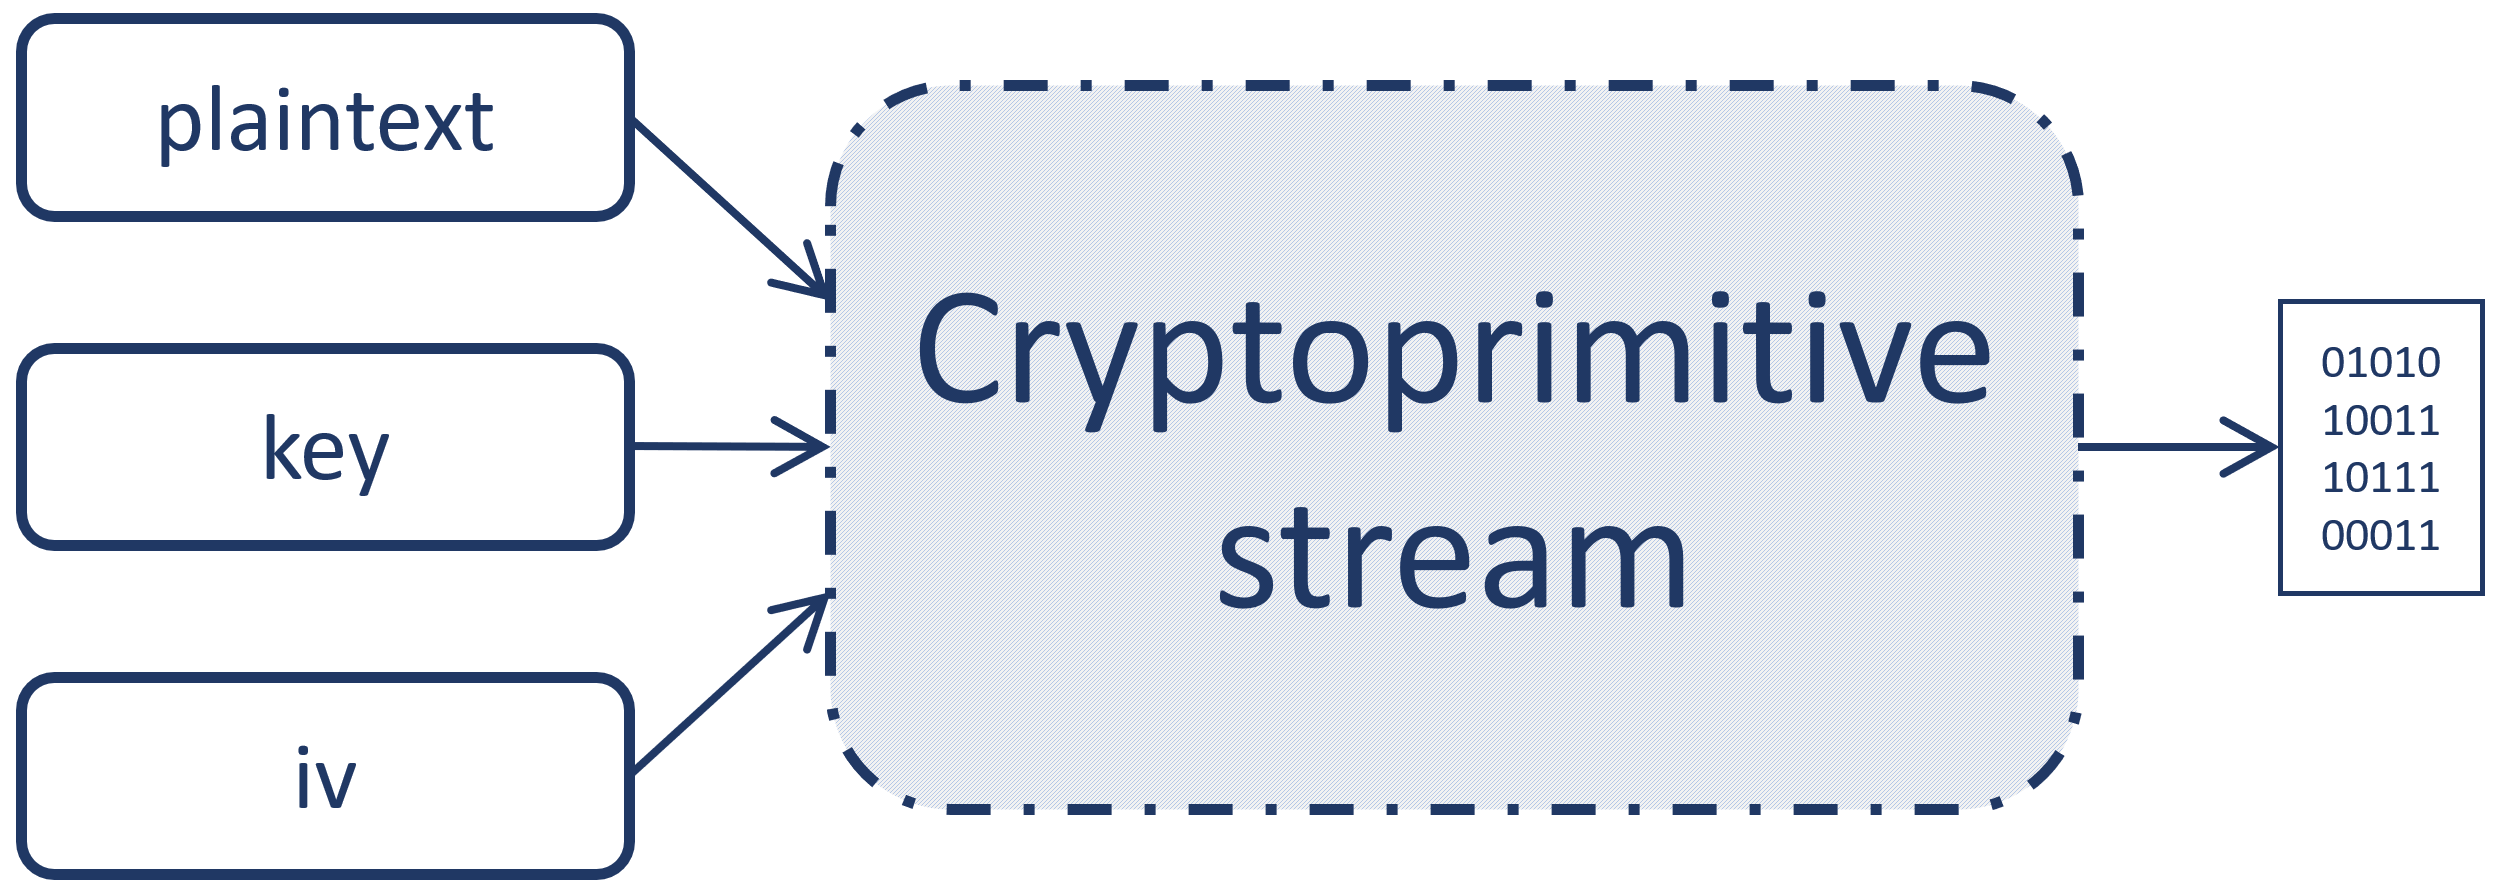
\includegraphics[width=0.7\textwidth]{./images/pictures/cryptoprimitive-stream.png}
		\caption{Example of one call of cryptographic primitive \textit{stream}, where used function is block cipher.}
		\label{fig:crypto-stream}
	\end{figure}
	
	\item[\textit{Streams} based on pseudo-random number generators.] Those \textit{streams} are newly introduced as part of this thesis. It is not possible to round-reduce those types of generators; this means the only way how to weaken those generators are to provide them seed with specific randomness properties for example with low Hamming weight. As \cref{fig:prng-streams} shows those streams are seeded in the beginning and then provide infinitely many output chunks. It is also possible to reseed generator after some specified number of \textit{chunks} generated. 
	
	All functions within this category are presented in \cref{sec:added_pseudo_random_generators}.
	
	\begin{figure}[h]
		\centering
		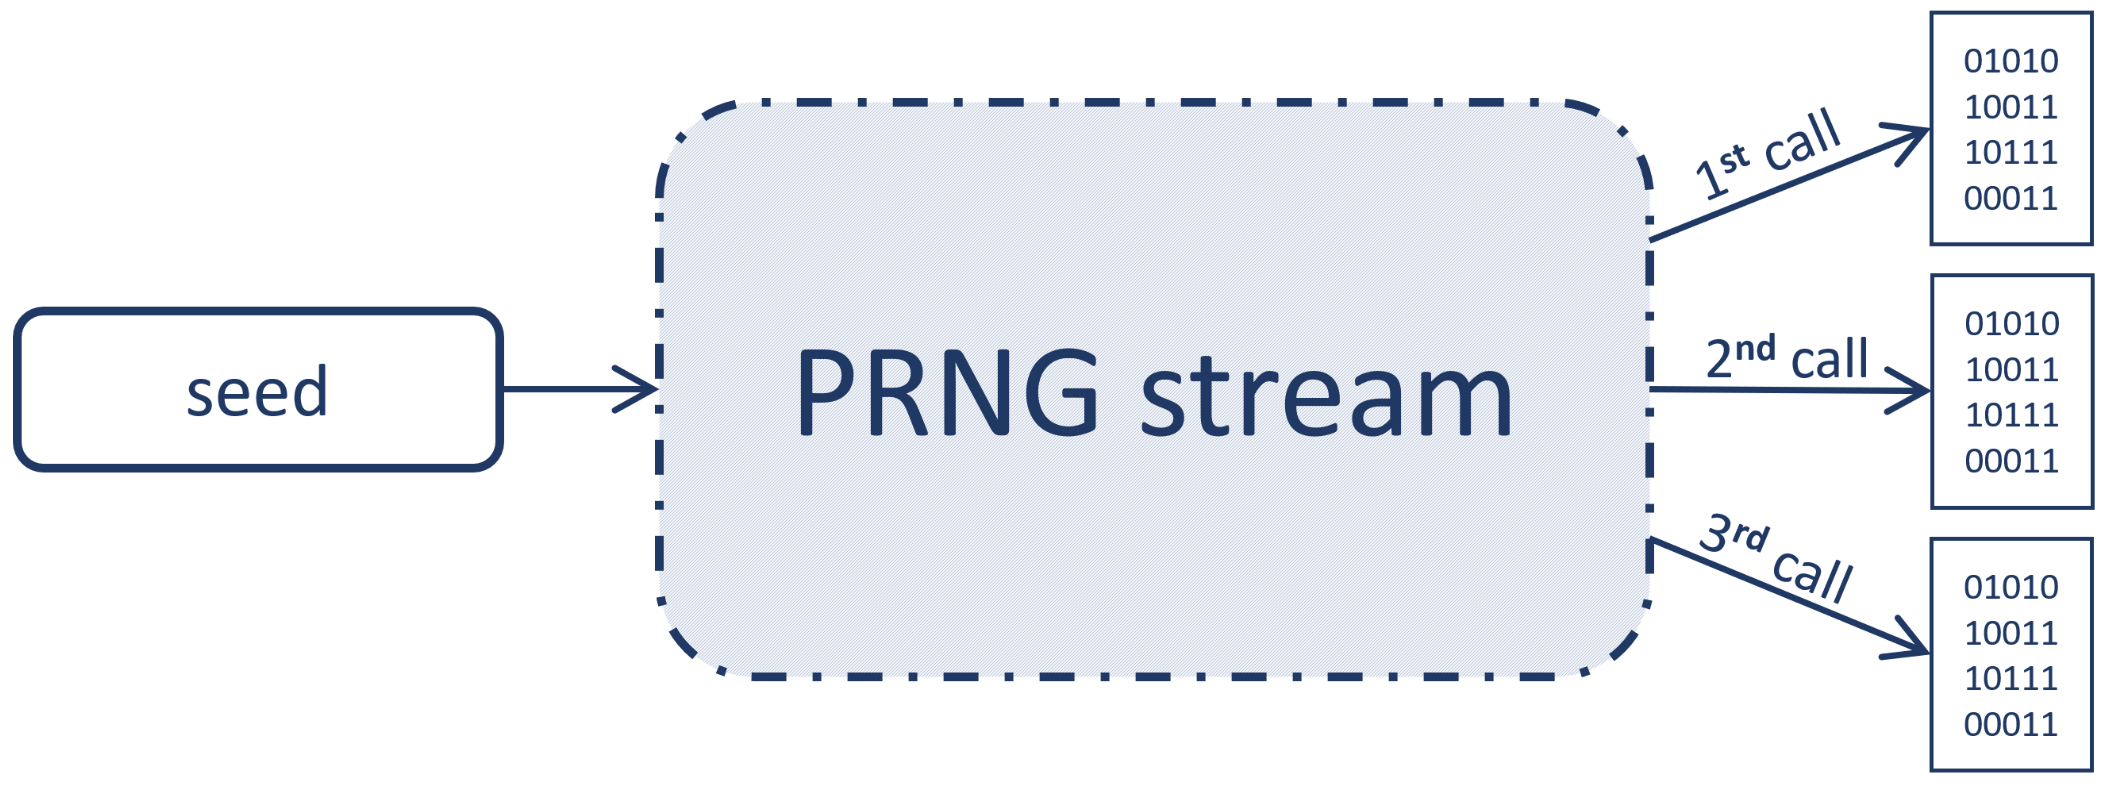
\includegraphics[width=0.7\textwidth]{./images/pictures/prng-stream.png}
		\caption{Example of three calls for a new chunk with same seed from pseudo-random generator \textit{stream}.}
		\label{fig:prng-streams}
	\end{figure}
	
\end{description}

Notice that all inputs are in the form of another \textit{stream}. Receiving \textit{stream} is deciding how much data and when will use from \textit{streams} on its input. For example, if receiving \textit{stream} is a cryptographic primitive type which requests new plaintext for each chunk (e.g., from input static stream), but the key is random and fixed for the whole generation. See the figure \cref{fig:config-schema} for an example of a scheme of the whole run of CryptoStreams. The middle block is the most important one. It is \textit{cryptographic primitive stream} and on its input it has 3 \textit{static streams}.

\begin{figure}[h]
	\centering
	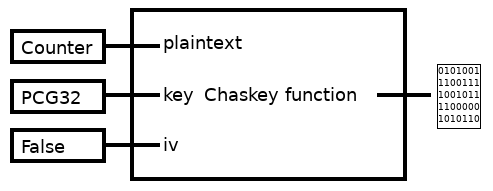
\includegraphics[width=0.7\textwidth]{./images/pictures/config-schema.png}
	\caption{Scheme of CryptoStreams configuration from \cref{fig:json-example}. More information about specific \textit{streams} within this picture can be found in \cref{subsec:configuration} }
	\label{fig:config-schema}
\end{figure}


\subsection{Configuration}
\label{subsec:configuration}

All necessary configuration within one run is achieved using a \texttt{JSON} file. Example of such configuration file can be found in \cref{fig:json-example} which will result in a file of size 8GB, generated from the AES function limited to 5 rounds. Key is generated pseudo-randomly using PCG32~\cite{pcgGen} at the beginning of a run and then used for generation of each output chunk. \textit{Counter stream} is used to generate plaintext blocks. Scheme of this configuration is shown in \cref{fig:config-schema}. 

The whole run of the generator is deterministic as it is using a pseudo-random generator with a specified seed. Experiments are therefore fully replicable using only stored \texttt{JSON} configuration. Notice that resulting file size is derived from \texttt{chunk\_size} in Bytes and \texttt{chunk\_count}. All possible options of configuration of CryptoStreams can be found in project documentation~\cite{CryptoStreams-wiki}.

\begin{figure}[h]
	\centering
	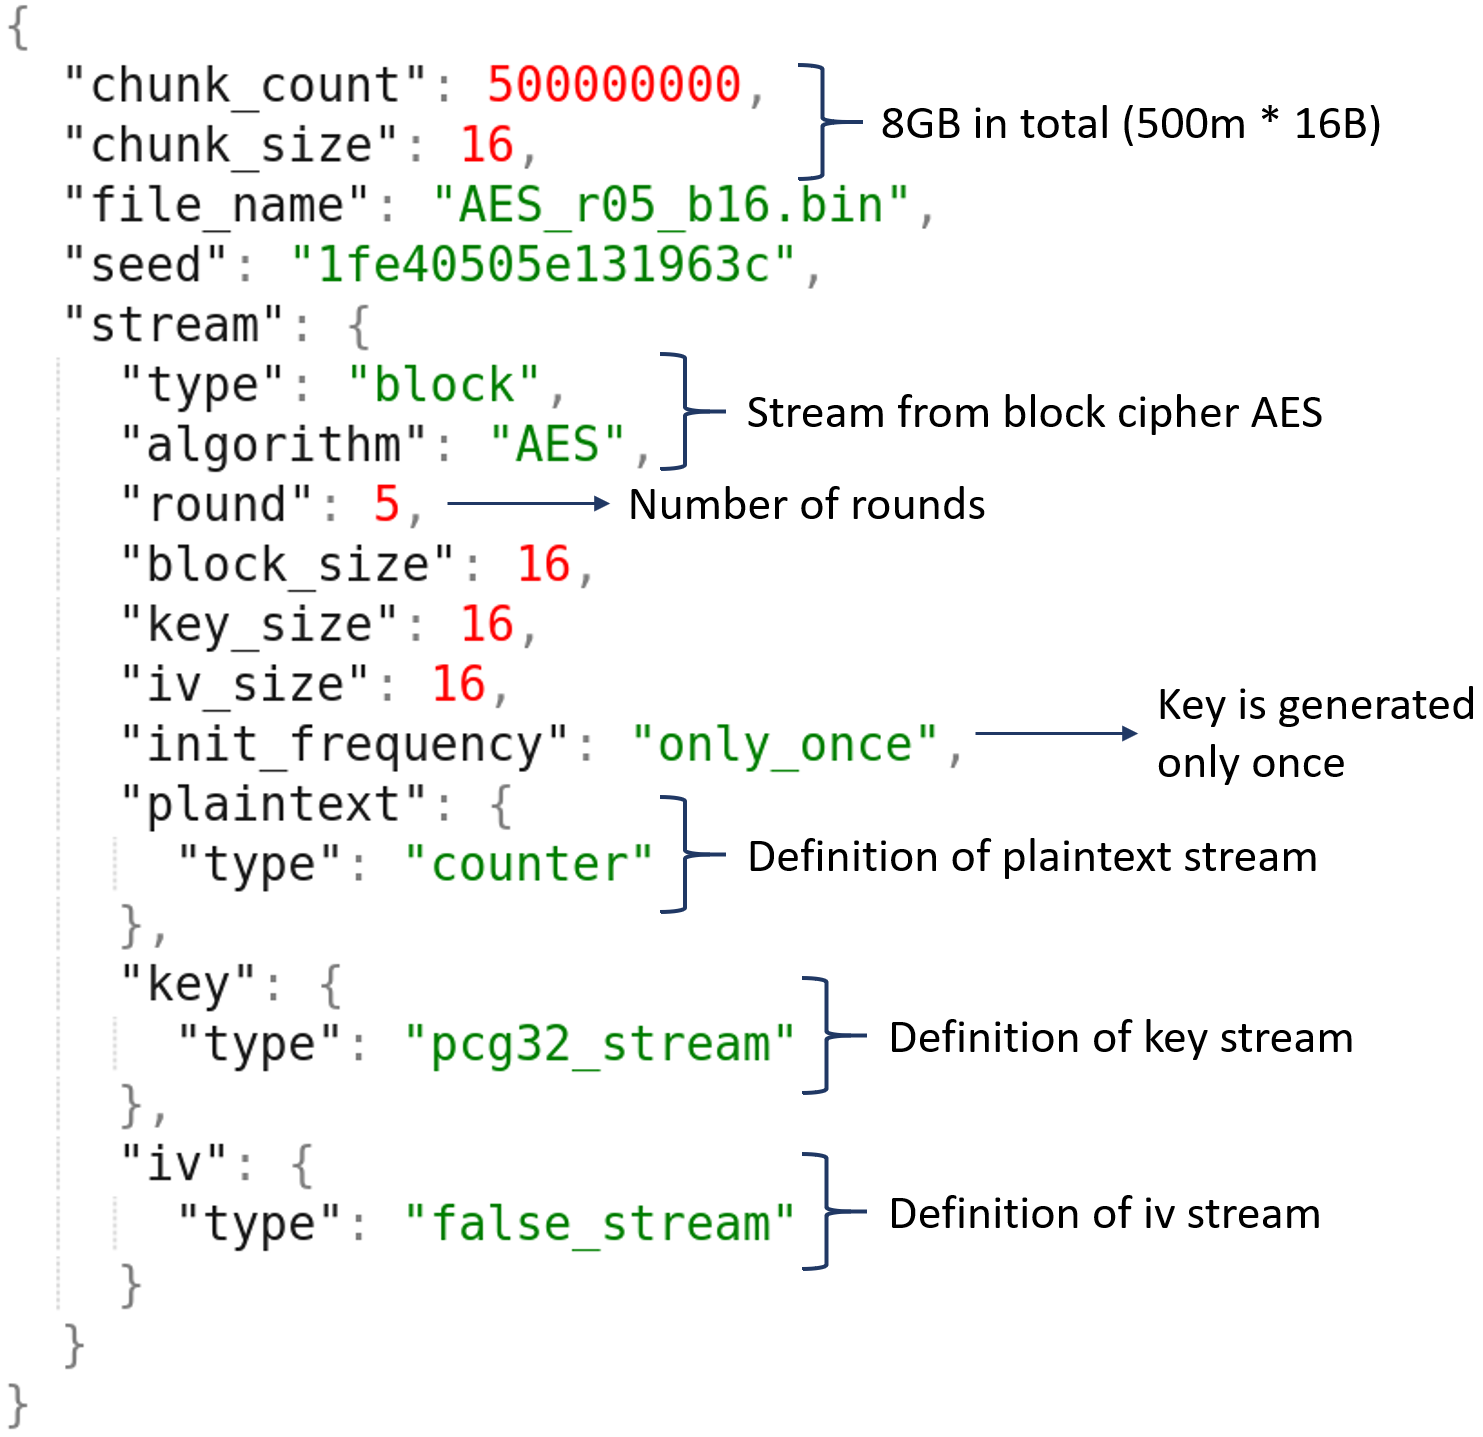
\includegraphics[width=0.7\textwidth]{./images/pictures/config.png}
	\caption{Example of \texttt{JSON} configuration for the tool CryptoStreams.}
	\label{fig:json-example}
\end{figure}


\subsection{Testing of streams}

Our statistical analysis relies on the fact that data which come from CryptoStreams are correct and genuinely come from cryptographic primitives. For that reason, we introduced testsuite which contains a various number of tests per individual \textit{stream}. We have added tests only for most frequently used \textit{streams}. Tests are also required for all newly added \textit{streams}. Results in this thesis are based on \textit{streams} which are tested.

As testing backend we are using Google Test~\footnote{\url{https://github.com/google/googletest}} framework. To ensure all tests are passing for each new change we use continuous integration tool called Travis CI\footnote{\url{https://travis-ci.org}}.

There are two things which are important to test First one is function itself, source code which is included within CryptoStreams. The other thing is CryptoStreams superstructure which encapsulates all cryptographic primitives and functions into one interface. Each type of \textit{streams} have different testing scenarios.

\begin{description}
	\item[Block ciphers \textit{streams}] are tested with test vectors in both directions, encrypt and decrypt. Also, both mentioned layers are tested. All those tests are testing function only in the full number of rounds as we were not able to find test vectors for round limited version. For lightweight cryptographic primitives based \textit{streams} we also added an \textit{encrypt-decrypt} test, for all supported rounds which is testing whether encryption of plaintext followed by decryption results with inputted plaintext. However, this test does not work for all added functions; the reasons are summarized in \cref{sec:added_lightweight_crypto}. Test coverage is complete for block ciphers with all 42 functions supplied with test vectors.
	
	\item[Hash functions \textit{streams}] are tested with test vectors in the full number of rounds. Both low-level function and CryptoStreams superstructure are included in tests. 29 out of 51 hash functions are covered with tests.
	
	\item[Stream ciphers \textit{streams}] are tested similarly as block ciphers except for encrypt-decrypt test for round reduced versions. From 27 stream ciphers 15 are tested.
	
	\item[Pseudo-random generators \textit{streams}] are hard to test, we have not found any test vectors. Nonetheless, we at least added test for linear generators by implementing an expected succession of numbers in tests and then compare whether we are getting same numbers from generator implementation. Four generators out of six included in CryptoStreams are tested. However, one test is testing only whether the generator is running without checking the correctness of output.
	
	\item[Other \textit{streams},] static or manipulating, are easy to test as we know how exactly should output look like.
	 
\end{description}
\begin{table}[t]
	\centering	
	\begin{tabular}{c|c c c c}
		\textbf{\large Crypto primitive type} &  Block ciphers &  Hash functions &  Stream ciphers &  PRNGS  \\ \hline
		\textbf{\large Tested/All functions} & 42/42	&	29/51		&		15/27	&		4/6	\\
		
	\end{tabular}
	\caption{List of all types of cryptographic primitives with the number of functions covered with tests.}
	\label{table:tested-cryptoprimitives}
\end{table}

\section{Conducted experiments}

The experiment we conducted was based on testing of randomness provided by functions in some extreme scenario. Either by the limitation of function rounds if it is available or by providing specific input. We tested the following scenarios.

\begin{description}
	\item[A specific type of input,] mostly with some lousy randomness properties, is provided to functions and statistical analysis is conducted where results are compared with random or other specific inputs. For this thesis, we used the following types of inputs.
	\begin{enumerate}
		\item Counter \textit{stream} is such \textit{stream} in which each chunk is the addition of one to the previous chunk in number representation.
		\item Low Hamming weight \textit{stream} returns outputs with least count of ones it is possible. Starting with all zeroes followed with only binary one on each position, two binary ones, etc.
		\item Strict avalanche criterion is a type of \textit{stream} in which the first chunk is randomly generated, and every next call is just previous chunk with one flipped bit.
	\end{enumerate}

	\item[Round reduction.] Almost every cryptographic function is build so that it performs a very same sequence of operations defined number of times, mostly in a loop. The number of times sequence should be performed is denoted by term \textit{number of rounds}. For example, AES~\cite{FIPS-197} has a recommended number of rounds 10, 12 or 14 based on key length as you can see in \cref{fig:fips197-rounds}. Each round in AES consists of \textit{SubBytes, ShiftRows, MixColumns, AddRoundKey} operations. The original implementation of AES has different key scheduling phase based on the number of rounds. However, we keep key scheduling in the full number of rounds for all functions in CryptoStreams so that we avoid some undefined behavior based on uninitialized parts of the key.
	
	\begin{figure}[h]
		\centering
		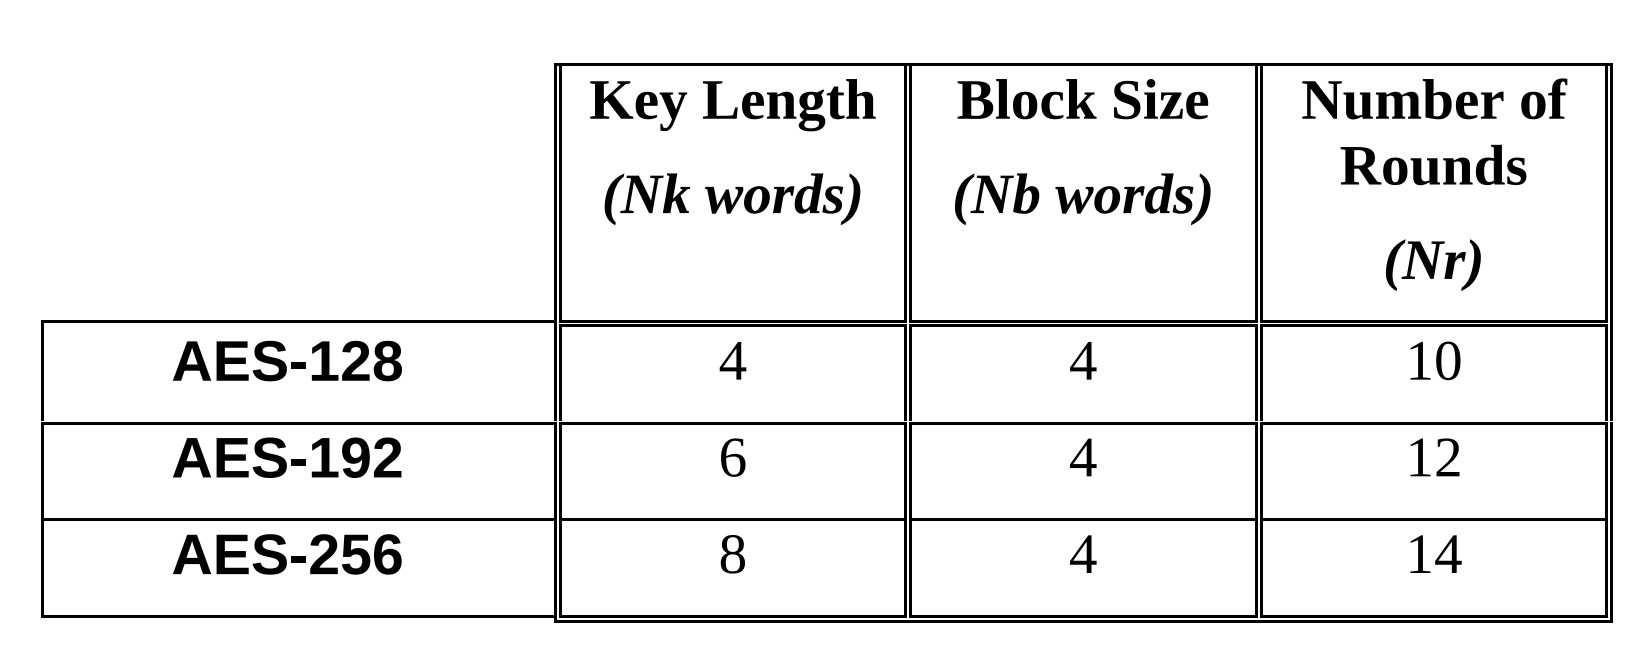
\includegraphics[width=0.4\textwidth]{./images/pictures/FIPS197-Nr-table.png}
		\caption{Table of rounds based on key size which is taken from~\cite{FIPS-197}, word size is 32 bits.}
		\label{fig:fips197-rounds}
	\end{figure}

	Authors of each cryptographic function specify how many rounds should be used to have reasonable security and performance. This number is called \textit{full number of rounds} and should be determined by conducting all known attacks against function limited to several numbers of rounds. Important indicator during this process is called \textit{security margin}. Security margin denotes the rate between round vulnerable to some cryptanalysis attack and the full number of rounds. For example, at the moment it is not possible to find any practical shortcut attack (any attack which is more efficient than exhaustive key search) for more than six rounds for AES with key length 128 bits. Therefore it is recommended to add four more rounds as a security margin and use AES with ten rounds \cite{daemen1999aes}. Notice that \textit{security margin} is not some general notion for the whole function, instead of that it is just kind of expression of resistance against particular cryptanalysis technique or attack.
	
	In this thesis, we investigate security margin based on indistinguishability of output of cryptographic primitive limited to all possible rounds from a random stream.
	
	\item[Plaintext ciphertext stream] produces pairs of input and output to function. With statistical testing performed on such output, it is possible to investigate dependency between plaintext and ciphertext. Since plaintext is part of the resulting sequence it is important to choose data with good randomness properties otherwise it may cause some interference in testing results.

\end{description}

\subsection{Testing with Randomness testing toolkit}

For running experiments, we are using a tool called randomness testing toolkit (RTT). It is a project which unifies more software tools for randomness testing under one interface. It provides both graphical interface (GUI) in the form of webpage and command line interface (CLI). CLI is mainly used for submission of a higher number of experiments due to possible automation, for example with python or shell scripts. Also GUI provides webpage form for submission of an experiment, but it is much easier to use CLI for automation. Besides the submission form, the webpage also provides an interpretation of results in a consistent way between all batteries. Three types of assessments OK, SUSPECT and FAIL are assigned to batteries based on the amount of failed test. The results of individual tests within batteries are evaluated with significance level $\alpha = 0.01$.

RTT contains tests from three software tools: {NIST STS}~\cite{nist-sts}, Dieharder~\cite{dieharder} and TestU01~\cite{l2007testu01}. We used all statistical batteries which RTT provides, except for Big Crush from TestU01 because it requires at least 60GB of data per run, which would be too demanding for resources. 

\subsection{Testing with BoolTest}

TODO: Using metacentrum? Info about runtime...

\section{Investigated pseudo-random generators}
\label{sec:added_pseudo_random_generators}

In this section, we will present all functions which were incorporated to CryptoStreams and then investigated for indistinguishability from the truly random stream.

\subsection{Pure pseudo-random generators}

The first part of this thesis is the addition to CryptoStreams and analysis of pure (do not use any cryptographic primitive to generate pseudo-randomness) pseudo-random number generators. It was not possible to round reduce those generators because the implementation does not provide it. Hence we only weakened them with seed with specific randomness properties. This component is quite small as we added together only six generators. The reason why we added such a small amount of generator is that we have not found any source of generators which would offer generators in a way it would be easy to incorporate to CryptoStream.

One of the sources of generators was a TestU01~\cite{l2007testu01} project. It contains a high number of generators, but they offer just implementations without parameters set up. So we needed to find out those parameters ourselves, and it was sometimes difficult to choose correctly. Reasons for difficulties was, for example, selecting parameters so that output was long enough to fill 8 bytes of data, absence of literature for less widely used generators, etc. We have taken over three generators and also included some basic tests. All generators are appropriately described in TestU01 user guide \cite{LEcuyer07testu01}.
\begin{description}
	\item[Linear congruential generator.] Definition of this generator is shown in \cref{formula:lcg}. Chosen parameters are taken from \cite{L-Ecuyer:LCG} and values are $a = 4645906587823291368$, $c = 0$ and $m = 9223372036854775783$. We have chosen as big parameter \textit{m} as possible because the generator is outputting values modulo this parameter, this means values are always less than this number. Since returning value from the generator is always 8 bytes long and the number $ 9223372036854775783 $ have few upper bits binary zeroes, also outputting value will always have those bits binary zero. For that reason, we cut those bits to not have any interference caused by too many zeroes in statistical tests. This is the main reason for adding such a small number of generators in this thesis because it would require too much configuration and testing to be sure the generators are working properly.
	
	\item[Multiple recursive generator.] Another linear generator, which is based on a very similar principle as LCG, with the difference that it combines data from more than one previous run. It is based on following formula.
	
	\begin{equation}
	x_{n} = \left(a_{1} \times x_{\left(n-1\right)} + . . . + a_{k} \times x_{\left(n-k\right)}\right)~~\bmod~~m
	\end{equation}
	
	Where \textit{k, $a_{1} .. a_{k}$ and m} are parameters of the generator hardcoded within CryptoStreams, $X_{n-l}$ is an output of a run $n-l$ where $n$ is current run and $l$ is a number between $1$ and $k$. The seed represents initial values of $X_{1}$ to $X_{k}$.
	
	 Chosen parameters are following: $ k = 2 $, $ a_{1} = 2975962250 $, $ a_{2} = 2909704450 $ and $ m = 9223372036854775783 $ \cite{L_Ecuyer:MRG}. We are cutting upper binary zeroes similarly like in LCG.
	
	\item[Xorshift generator.] The generator is based on \textit{xor} and \textit{shift} operations~\cite{RePEc:jss:jstsof:v:008:i14}. We have chosen version which is created by function \texttt{uxorshift\_CreateXorshift13} and requires no additional parameters, more information in \cite{LEcuyer07testu01} on page 50. \\
\end{description}

The second source of pseudo-random streams is the standard library of C++. Unlike TestU01 it contains generators including parameters. It is less complicated to take over this code as it is enough to use \texttt{include} directive. The only disadvantage of this source is it contains only three pseudo-random generators. List of generators is following.

\begin{description}
	\item[Linear congruential generator~\footnotemark.] The same generator as we have taken over from TestU01. The definition is shown in \cref{formula:lcg}. Used parameters are $a = 48271$, $c = 0$ and $m = 2147483647$. As you can see numbers are much smaller, than those we have chosen for the generator from TestU01. The reason is that this generator outputs only 4 Bytes instead of 8 Bytes. 
\end{description}
	
	\footnotetext{\url{https://en.cppreference.com/w/cpp/numeric/random/linear\_congruential\_engine}}
	
\begin{description}
	\item[Mersenne Twister~\footnotemark.] The generator was developed by Makoto Matsumoto and Takuji Nishimura \cite{Matsumoto:1998:MTE:272991.272995}. However, it does not produce cryptographically secure random numbers \cite{jakobsson2014theory}. 
	
\end{description}

\footnotetext{\url{https://en.cppreference.com/w/cpp/numeric/random/mersenne\_twister\_engine}}

\begin{description}

	\item[Substract with carry~\footnotemark.] This type of generator was introduced by George Marsaglia and Arif Zaman \cite{marsaglia1991}. The definition is following:
	
	\begin{equation}
	x_{n} = \left(x_{n-S} - x_{n-R} - cy(n-1)\right)~~\bmod~~M
	\end{equation}
	Where 
	
	\begin{equation}
	cy(n) = \begin{cases}
	1, & \text{if } x_{n-S} - x_{n-R} - cy(n-1) < 0\\
	0, & \text{otherwise}
	\end{cases}
	\end{equation}
	and \textit{S,R} are parameters hardcoded in CryptoStreams. $x_{k}$ represents $k$-th output of the generator. The seed represents initial values of $x_{1}$ to $x_{k}$ where $k = max{R, S}$.
	
\end{description}

\footnotetext{\url{https://en.cppreference.com/w/cpp/numeric/random/subtract\_with\_carry_engine}}

\subsection{Generators based on lightweight cryptographic primitives}
\label{sec:added_lightweight_crypto}

The other part contains block ciphers taken over from project FELICS~\cite{dinu2015felics} developed by Daniel Dinu and his group at the University of Luxembourg. This project is conducting a performance analysis of lightweight functions that are intended for embedded devices. We have taken over only the C++ implementation of functions, as we were not interested in implementations optimized for other architectures. We needed to implement round reduction of functions ourselves as the project contained only full round implementation. However, provision of round reduction was mostly straightforward as functions were prepared with round reduction in mind and we only needed to replace constant in a loop with a variable which is configurable from CryptoStreams. 

Besides the main loop, functions mostly contain also key scheduling, initial and final part. Key scheduling is taking care of the creation of round keys based on a provided key. Initial and final part serves for initialization and finalization of the process. We do not round-reduce any of those parts as we wanted to avoid some memory problems like uninitialized or wrongly cleaned memory.

\cref{table:list-of-investigated functions} contains all investigated functions including some basic information about them. Our intention was also adding two test scenarios, for testing correctness of implementation, for each added function. 

The first scenario is testing all functions with test vectors in full number of rounds. Test vectors were taken over from project FELICS. 

The second test scenario is verifying the expected functionality of round-reduction by doing encryption followed by decryption (Encrypt-Decrypt test) for all rounds provided by tested function. This test is not passing for 6 functions out of 19 (failing marked with \textit{\xmark} in last column in \cref{table:list-of-investigated functions}). The possible explanation of failure is missing round-reduction of key scheduling, which we intentionally do not perform. Despite the failure of the test we observed expected behavior concerning detectable bias by statistical testing - more rounds results in less bias.

\begin{table}[t]
	\centering
	\begin{tabular}{c|c c c c}
		\textbf{\large Function} & \textbf{\large Round} & \textbf{\large Block size} & \textbf{\large Key size} & \textbf{\large Encrypt-Decrypt test}\\ \hline
		Chaskey~\cite{cryptoeprint:2014:386}				& 16	& 16	& 16	& \cmark	\\ \hline
		Fantomas~\cite{grosso2014ls}						& 12	& 16	& 16	& \cmark 	\\ \hline
		HIGHT~\cite{10.1007/11894063_4}						& 32	& 8		& 16	& \xmark 	\\ \hline
		LBlock~\cite{10.1007/978-3-642-21554-4_19}			& 32	& 8		& 10	& \xmark \\ \hline
		LEA~\cite{Hong2013LEAA1}							& 24	& 16	& 16	& \xmark \\ \hline
		LED~\cite{Guo:2011:LBC:2044928.2044958}				& 48	& 8		& 10	& \cmark \\ \hline
		Piccolo~\cite{10.1007/978-3-642-23951-9_23}			& 25	& 8		& 10	& \cmark \\ \hline
		PRIDE~\cite{10.1007/978-3-662-44371-2_4}			& 20	& 8		& 16	& \xmark  \\ \hline
		PRINCE~\cite{10.1007/978-3-642-34961-4_14}			& 12	& 8		& 16	& \cmark \\ \hline
		RC5-20~\cite{10.1007/3-540-60590-8_7}				& 20	& 8		& 10	& \cmark \\ \hline
		RECTANGLE-K80~\cite{Zhang2015}						& 25	& 8		& 16	& \xmark \\ \hline
		RECTANGLE-K128~\cite{Zhang2015}						& 25	& 8		& 16	& \xmark \\ \hline
		RoadRunneR-K80~\cite{10.1007/978-3-319-29078-2_4}	& 10	& 8		& 10	& \cmark \\ \hline
		RoadRunneR-K128~\cite{10.1007/978-3-319-29078-2_4}	& 12	& 8		& 16	& \cmark \\ \hline
		Robin~\cite{grosso2014ls}							& 16	& 16	& 16	& \cmark \\ \hline
		RobinStar~\cite{grosso2014ls}						& 16	& 16	& 16	& \cmark \\ \hline
		SPARX-B64~\cite{10.1007/978-3-662-53887-6_18}		& 8		& 8		& 16	& \cmark \\ \hline
		SPARX-B128~\cite{10.1007/978-3-662-53887-6_18}		& 8		& 16	& 16	& \cmark \\ \hline
		TWINE~\cite{twine}									& 35	& 8		& 10	& \cmark \\ \hline
		
		
	\end{tabular}
	\caption{List of all investigated functions, where sizes are given in Bytes. Including information whether encrypt decrypt test passed.}
	\label{table:list-of-investigated functions}
\end{table}



\chapter{Results of evaluation of statistical randomness properties}


%%bibliography

\printbibliography[heading=bibintoc] %% Print the bibliography.

\appendix{}

\chapter{Glossary}
\label{chap:app-glos}


\end{document}
